% Build the update pages from this directory:
%   xelatex -interaction=nonstopmode -halt-on-error CB_pricing_update_20260828.tex
% Run XeLaTeX twice, then prepend the resulting PDF to
% HISTORICAL_BASE_20260310.pdf to produce CB_pricing_full.pdf.
\documentclass[11pt,a4paper]{ctexart}

\usepackage[a4paper,margin=2.1cm,headheight=14pt]{geometry}
\usepackage{booktabs}
\usepackage{fancyhdr}
\usepackage{graphicx}
\usepackage{hyperref}
\usepackage{tabularx}
\usepackage[table]{xcolor}
\usepackage{enumitem}

\definecolor{navy}{HTML}{17365D}
\definecolor{blue}{HTML}{2F5597}
\definecolor{lightblue}{HTML}{D9EAF7}
\definecolor{lightgray}{HTML}{F2F4F7}
\definecolor{muted}{HTML}{5B6573}

\hypersetup{
  colorlinks=true,
  linkcolor=blue,
  urlcolor=blue,
  pdfauthor={Convertible Bond Pricing Research},
  pdftitle={中国可转债绝对定价研究与实证比较}
}

\pagestyle{fancy}
\fancyhf{}
\lhead{\textcolor{muted}{中国可转债绝对定价研究}}
\rhead{\textcolor{muted}{数据截至 2026-08-28}}
\cfoot{\thepage}

\setlength{\parindent}{2em}
\setlength{\parskip}{0.35em}
\setlist[itemize]{leftmargin=2em,itemsep=0.25em}

\newcommand{\sectionbar}[1]{%
  \vspace{0.4em}
  {\color{navy}\Large\bfseries #1}\par
  \vspace{0.2em}
  {\color{blue}\rule{\textwidth}{1.2pt}}\par
}

\begin{document}

\begin{titlepage}
  \centering
  \vspace*{2.1cm}
  {\color{navy}\Huge\bfseries 中国可转债绝对定价研究\par}
  \vspace{0.45cm}
  {\color{blue}\LARGE 三模型定价、错误定价信号与组合检验\par}
  \vspace{0.9cm}
  {\Large 面向可复现证据的实证研究\par}
  \vspace{1.5cm}

  \renewcommand{\arraystretch}{1.45}
  \begin{tabular}{>{\bfseries}rl}
    数据截止日： & 2026-08-28 \\
    回测区间： & 2019-01-25 至 2026-08-28 \\
    调仓频率： & 月末调仓，共 91 个收益观察期 \\
    更新日期： & 2026-08-30 \\
  \end{tabular}

  \vfill
  \begin{minipage}{0.88\textwidth}
    \small\color{muted}
    本更新页以仓库内已生成并交叉核对的模型输出、策略结果和图表为依据。
    后附 2026-03-10 版本的完整研究正文，用于保留理论推导与历史研究框架；
    若历史正文中的回测数字与本更新页不一致，以本更新页为准。
  \end{minipage}
\end{titlepage}

\sectionbar{一、研究问题与贡献}

可转债同时具有债券现金流、股票期权和路径依赖条款。市场价格偏离理论价值时，
偏离可能来自模型遗漏、条款影响或可交易的信息。本研究在统一的数据与回测口径下
比较三种复杂度不同的绝对定价模型，并检验模型价格能否形成扣除交易成本后仍有
解释力的横截面信号。数据截至 \textbf{2026-08-28}。

\begin{itemize}
  \item \textbf{BS 模型：}闭式期权定价框架，主要反映正股价格、波动率、
        无风险利率与剩余期限对转债价值的影响。
  \item \textbf{ZL 模型：}基于蒙特卡罗路径并纳入已观测赎回、回售条款状态，
        同时使用信用利差对现金流折现。
  \item \textbf{LSM 模型：}使用最小二乘回归估计继续持有价值，
        比较即时转股与继续价值，并与 ZL 条款价值做稳健组合。
\end{itemize}

研究贡献包括模型比较与研究工程两个层面。定价误差和组合表现被分别检验，
避免把拟合改善直接解释为投资优势。数据、周度定价、因子、月度组合和发布流程
由同一套可复现管道衔接。ZL 与 LSM 使用独立 Manifest 验证历史输入与已发布输出，
完成历史初始化后，日常任务严格只计算新增交易周。

\begin{table}[h]
  \centering
  \caption{最新回测结果：六因子等权多头组合（含双边 0.06\% 交易成本）}
  \rowcolors{2}{lightgray}{white}
  \begin{tabular}{lrrrrr}
    \toprule
    模型 & 年化超额 & 夏普比率 & 最大回撤 & 年化波动 & 平均换手率 \\
    \midrule
    BS & 12.25\% & 0.91 & -28.96\% & 19.09\% & 54.33\% \\
    ZL & 13.40\% & 0.94 & -29.75\% & 19.78\% & 57.34\% \\
    LSM & 13.30\% & 0.92 & -31.04\% & 20.03\% & 55.23\% \\
    \bottomrule
  \end{tabular}
\end{table}

同期中证转债基准年化收益为 \textbf{7.08\%}。LSM 在定价偏差上改善明显，
但策略收益未稳定超越 ZL，最大回撤也更高。更好的定价拟合没有机械地转化为
更强的投资结果，这是本研究最重要的实证判断。三类组合均经历较大回撤，
因此定价信号不应被视为独立的低风险套利。

\sectionbar{二、定价结果与最新截面}

截至 2026-08-28，BS 模型有 313 只有效定价，ZL 与 LSM 均有 301 只。
在各自有效样本上，理论价格相对市场价格偏离度的截面中位数分别为
\textbf{-6.14\%}、\textbf{-17.83\%} 与 \textbf{-9.44\%}。LSM 将全样本平均偏差从 ZL 的
-12.85 元收窄到 -2.32 元，MAPE 由 9.49\% 降至 9.23\%。当前模型仍普遍给出
低于市场价格的估值，但不能直接解释为可无摩擦做空的套利空间：流动性、
信用风险、条款执行意愿、波动率估计误差和卖空约束都会影响偏离的可交易性。

\begin{figure}[p]
  \centering
  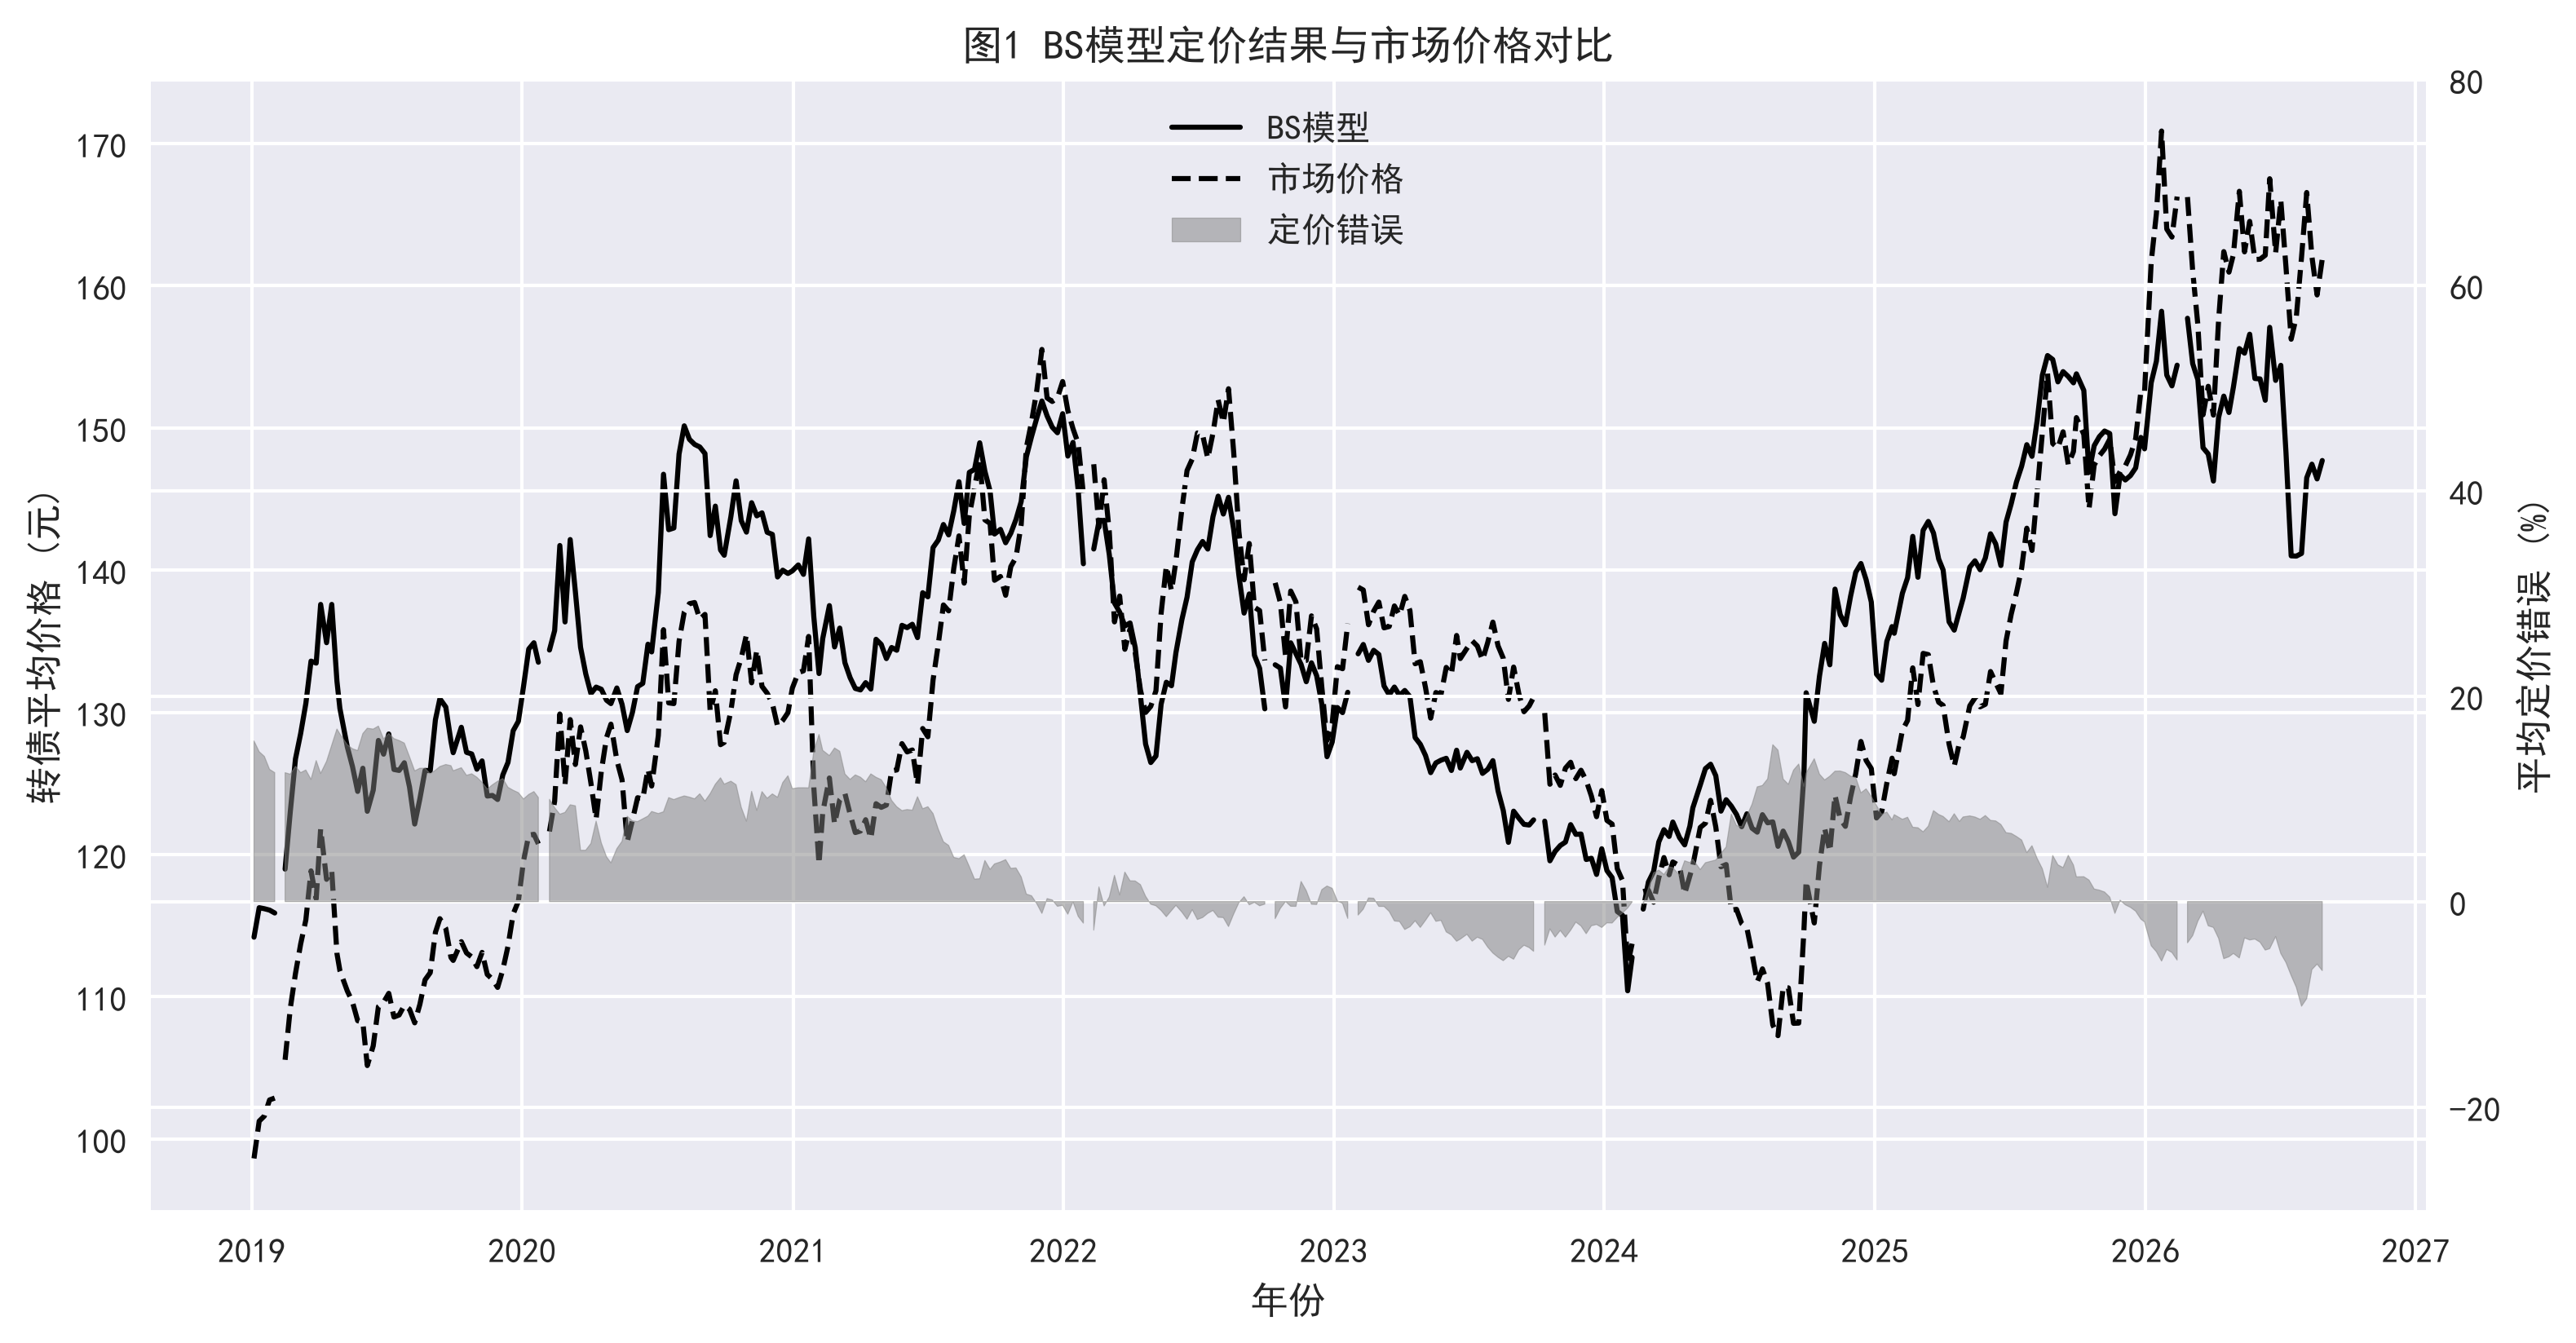
\includegraphics[width=0.76\textwidth]{../backtest/Fig1_BS_Price_Time_Series.png}
  \caption{BS 模型理论价格、市场价格与相对偏离度}
  \vspace{0.8cm}
  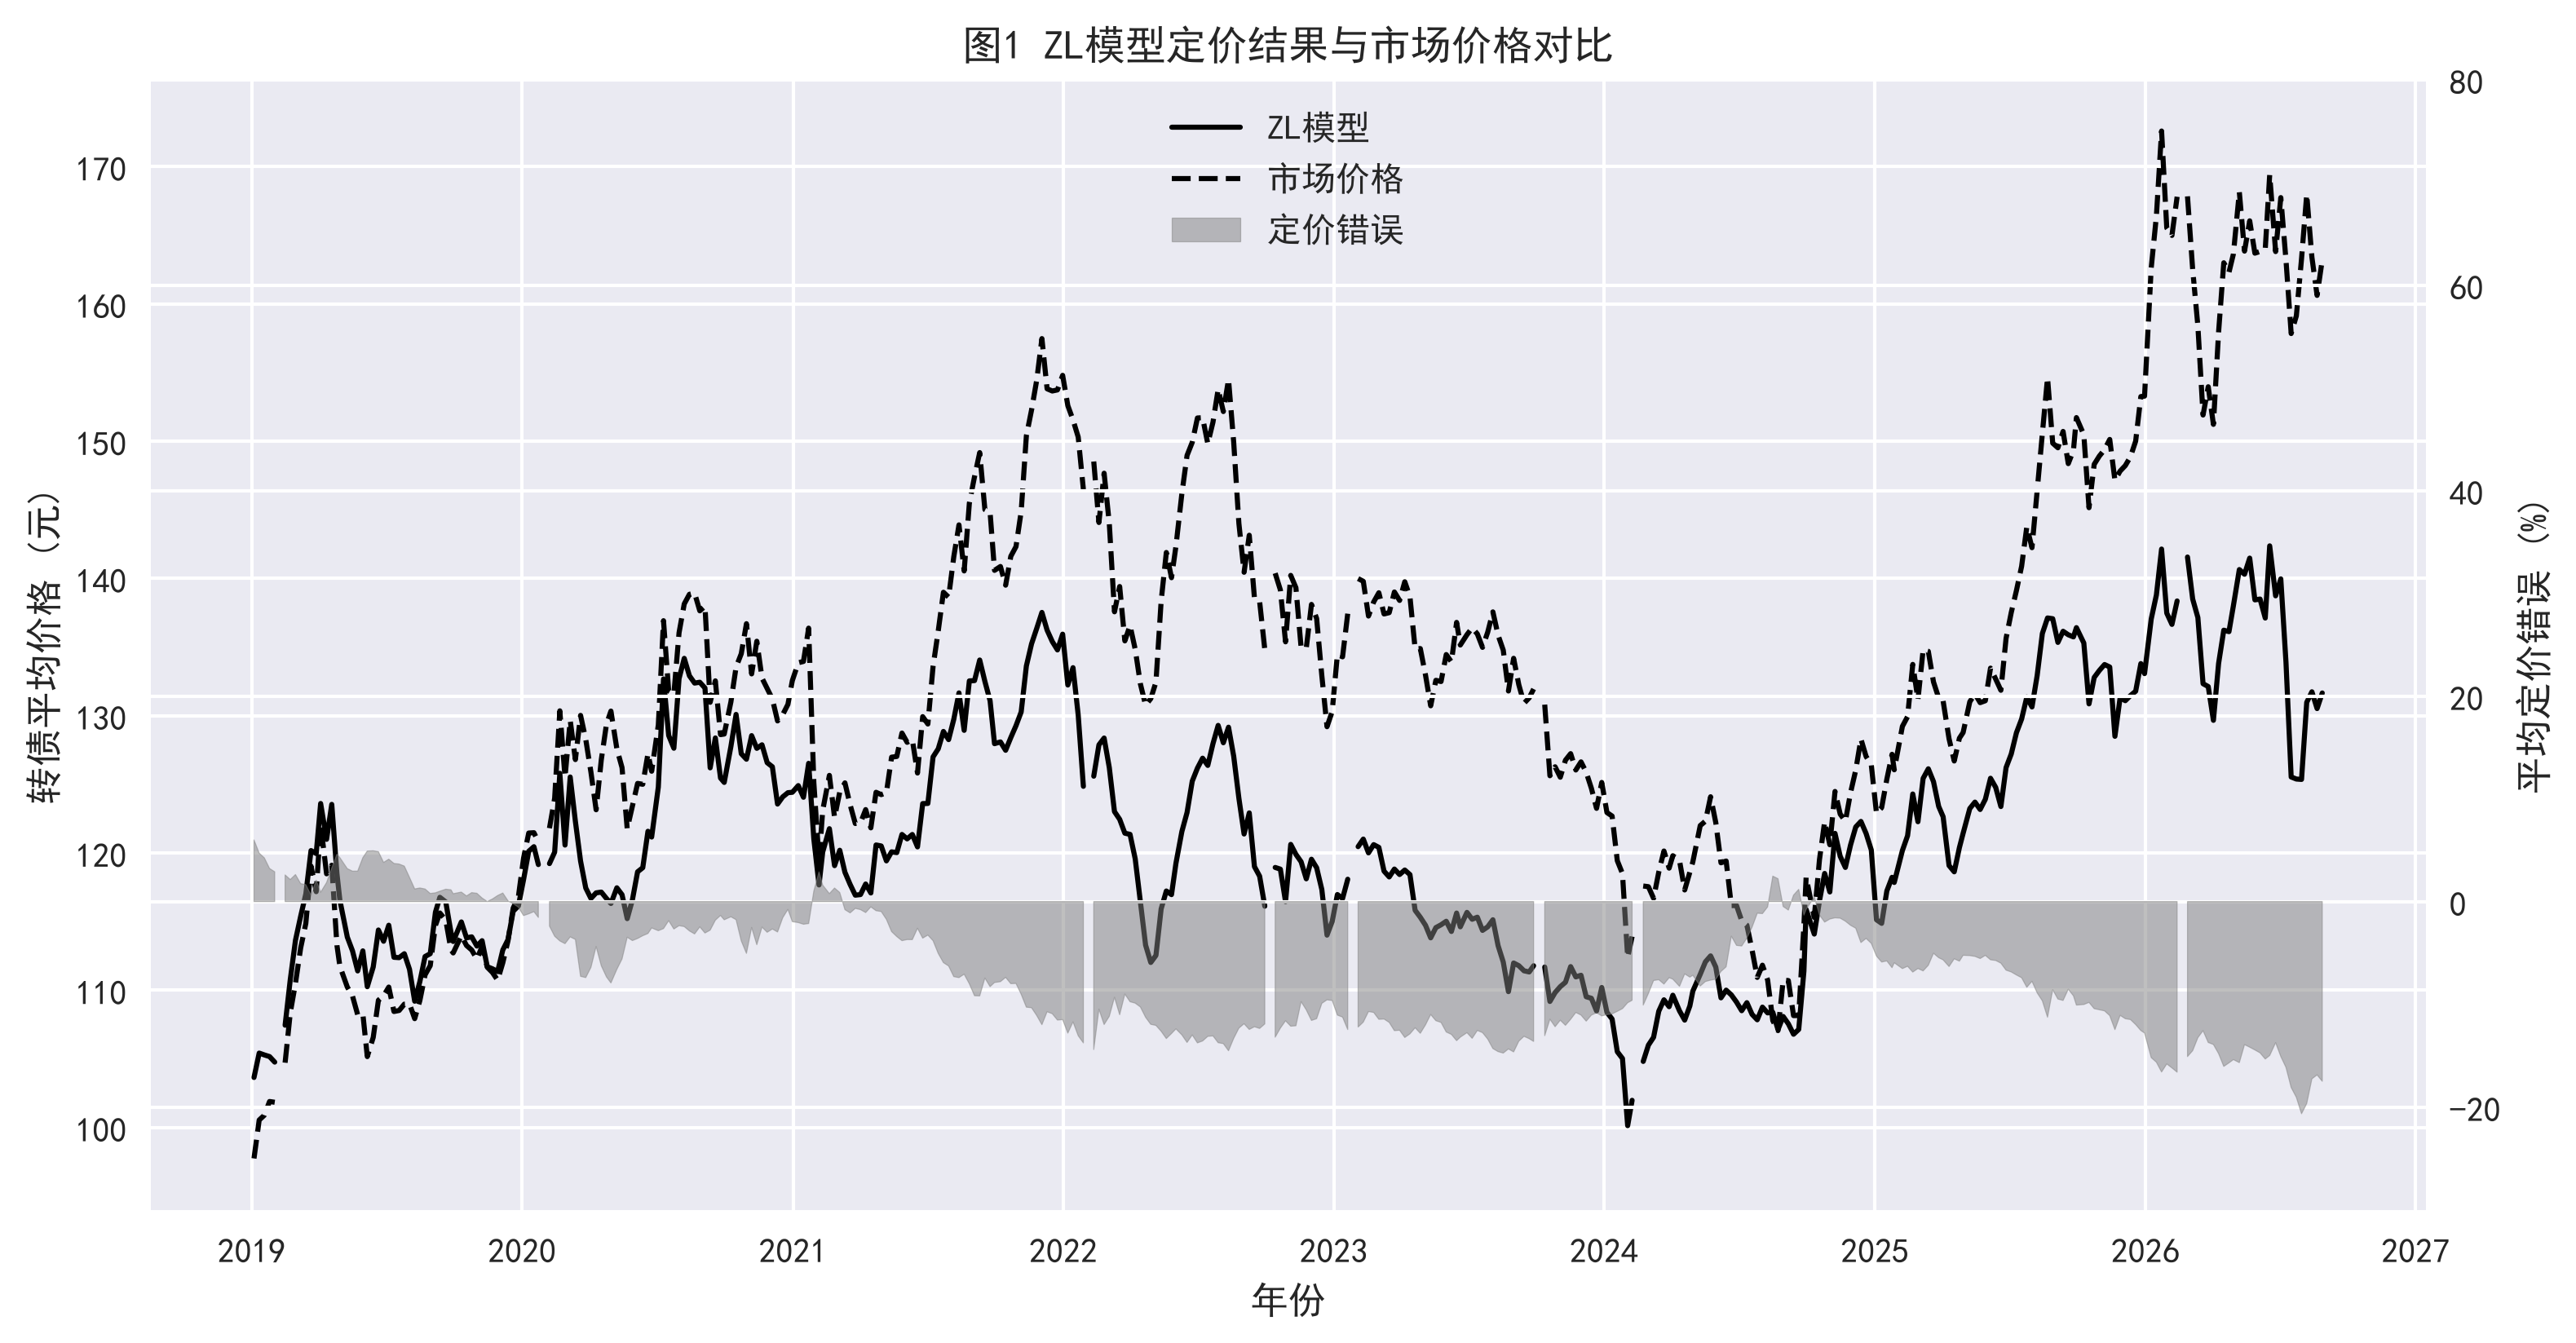
\includegraphics[width=0.76\textwidth]{../backtest/Fig1_ZL_Price_Time_Series.png}
  \caption{ZL 模型理论价格、市场价格与相对偏离度}
  \vspace{0.5cm}
  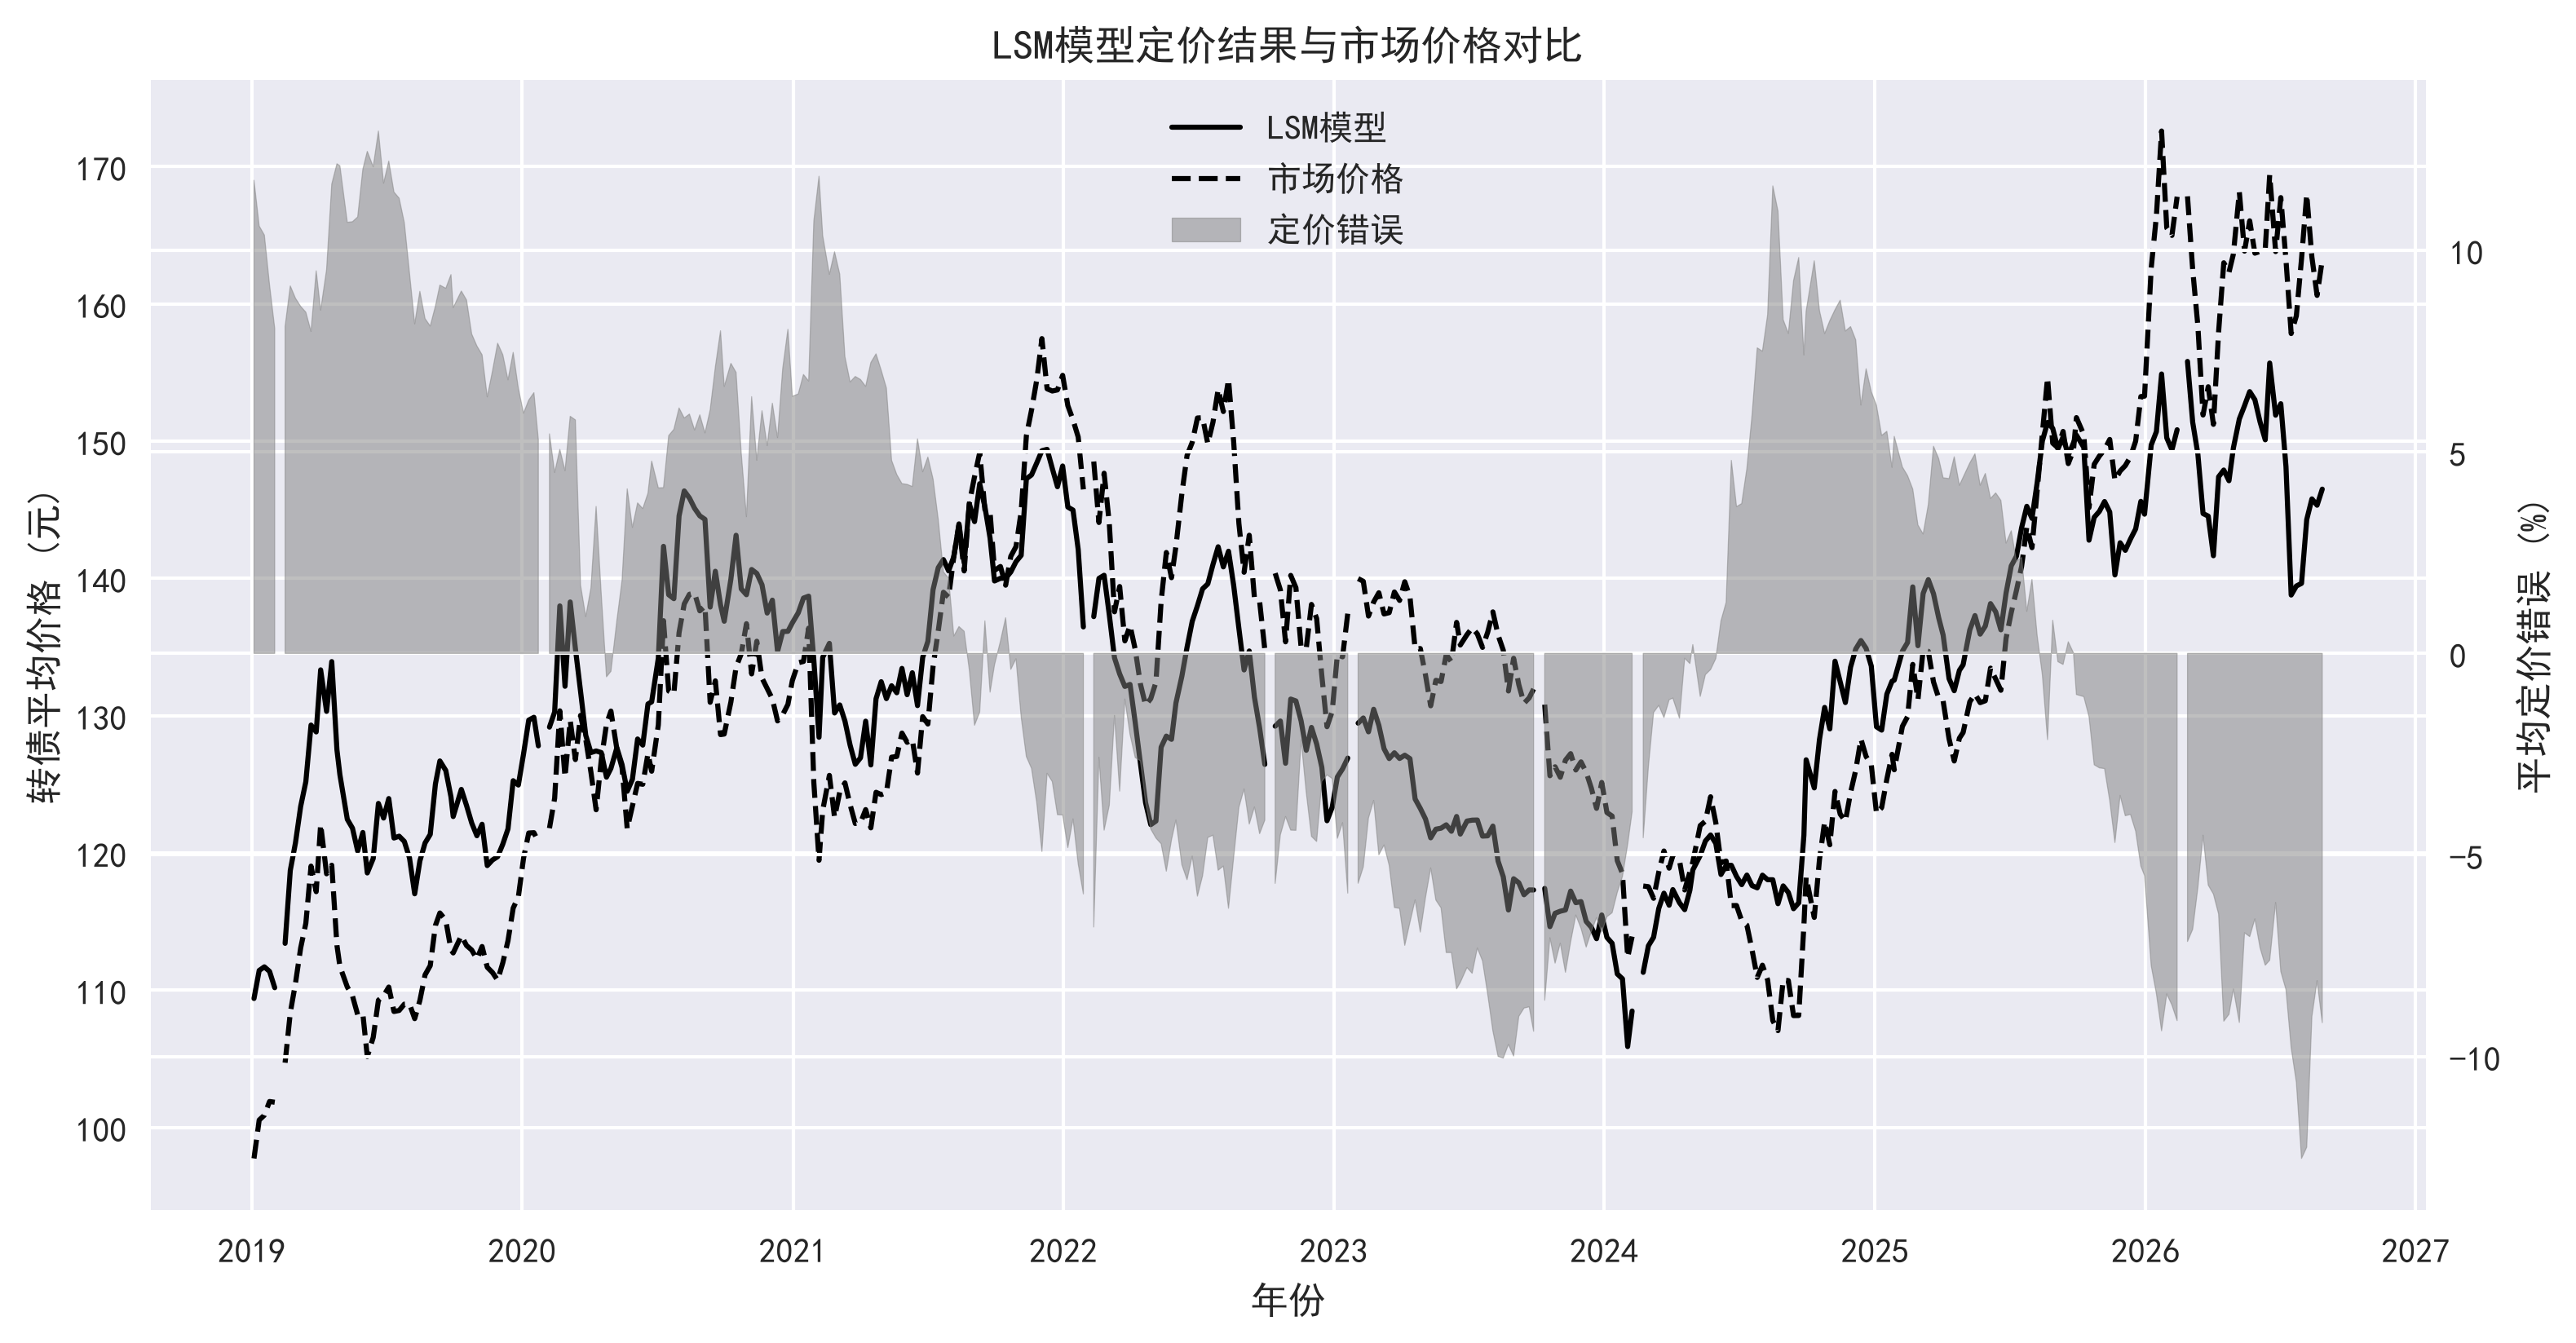
\includegraphics[width=0.76\textwidth]{../backtest/Fig1_LSM_Price_Time_Series.png}
  \caption{LSM 模型理论价格、市场价格与相对偏离度}
\end{figure}

\clearpage
\sectionbar{三、策略表现}

策略每月按六个标准化因子等权合成后选取多头组合。六个因子包括流动性、
波动率、量价相关性、估值、动量和相应模型的定价偏差。收益结果使用月度
持有期收益，并扣除双边 0.06\% 交易成本。

\begin{table}[h]
  \centering
  \caption{定价偏差单因子与六因子合成结果}
  \rowcolors{2}{lightgray}{white}
  \begin{tabular}{llrrrr}
    \toprule
    模型 & 策略 & 年化收益 & 夏普比率 & 最大回撤 & 累计收益 \\
    \midrule
    BS & 定价偏差单因子 & 13.26\% & 1.20 & -21.76\% & 239.61\% \\
    BS & 六因子等权 & 12.25\% & 0.91 & -28.96\% & 214.34\% \\
    ZL & 定价偏差单因子 & 15.22\% & 1.37 & -14.99\% & 292.88\% \\
    ZL & 六因子等权 & 13.40\% & 0.94 & -29.75\% & 243.23\% \\
    LSM & 定价偏差单因子 & 11.71\% & 1.14 & -20.82\% & 201.37\% \\
    LSM & 六因子等权 & 13.30\% & 0.92 & -31.04\% & 240.50\% \\
    \bottomrule
  \end{tabular}
\end{table}

定价偏差单因子在当前样本中的风险调整后表现优于六因子等权组合，尤其是
ZL 定价偏差因子。LSM 多因子组合的年化超额与 ZL 接近，但回撤更大。
这些结果来自同一历史样本内的描述性回测，尚不构成
样本外稳健性或未来收益保证。

\begin{figure}[p]
  \centering
  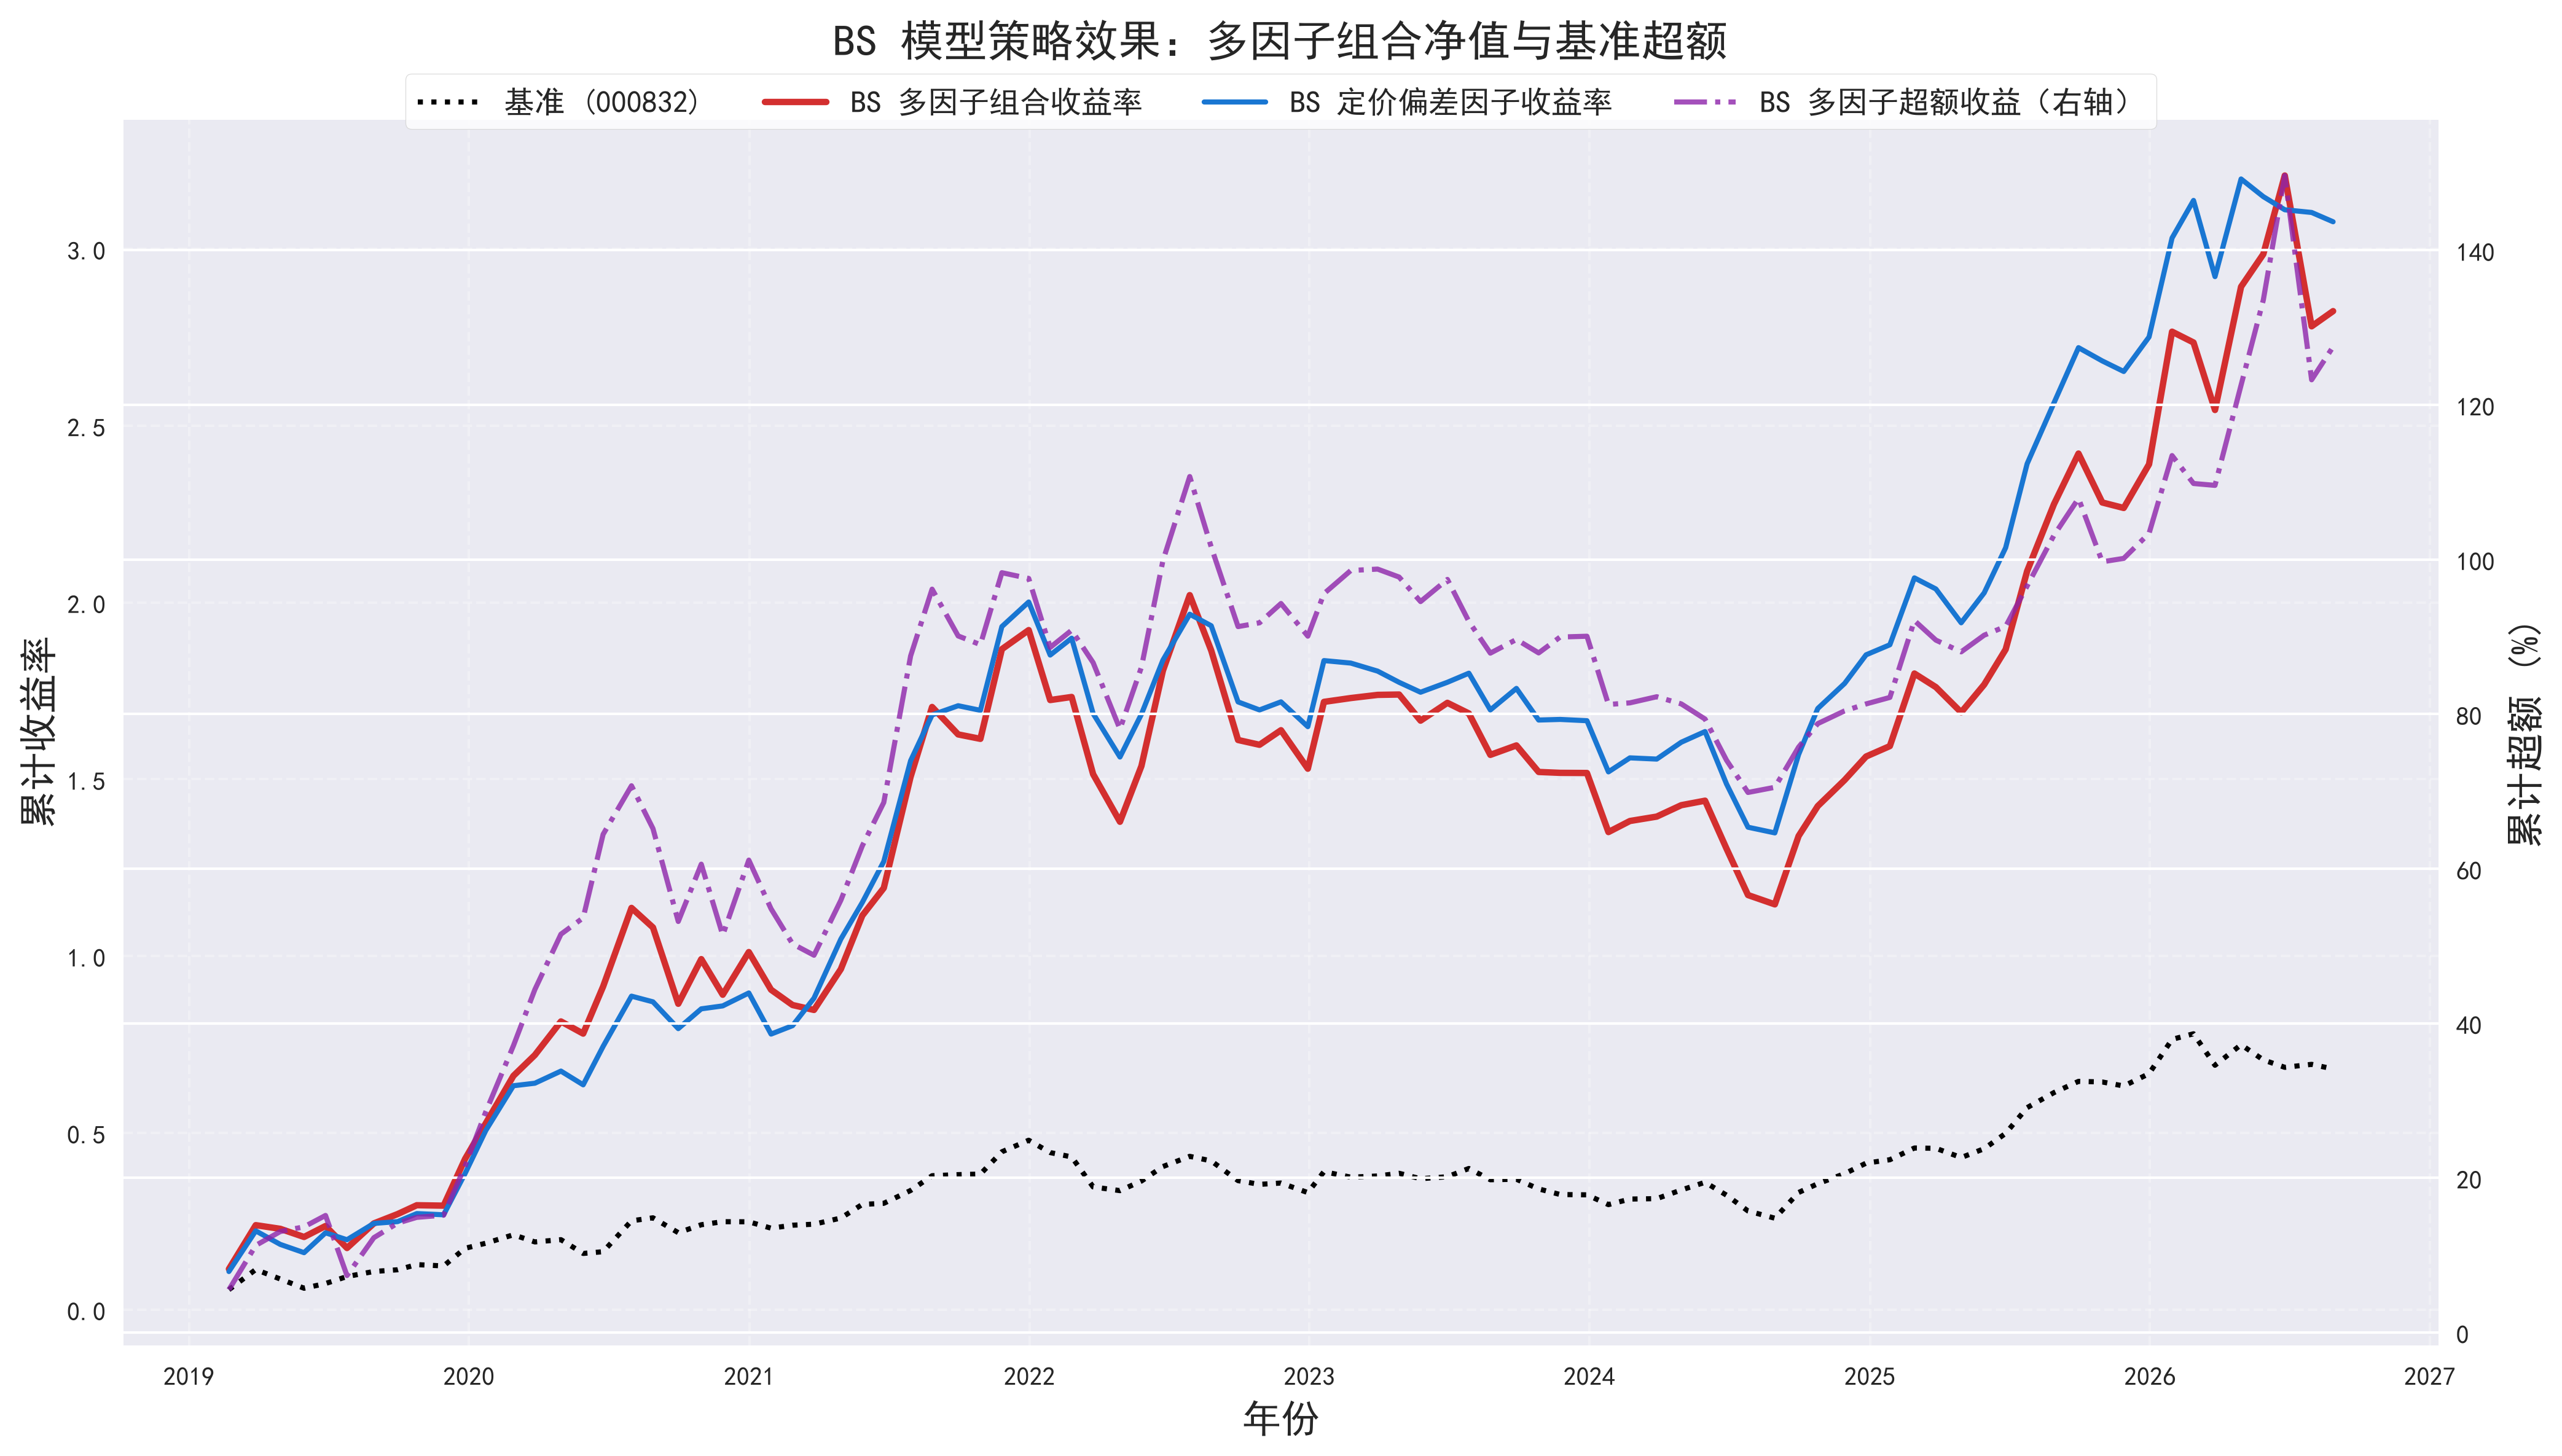
\includegraphics[width=0.76\textwidth]{../long-short strategy/BS_model_performance.png}
  \caption{BS 定价偏差策略与基准净值}
  \vspace{0.8cm}
  \includegraphics[width=0.76\textwidth]{../long-short strategy/ZL_model_performance.png}
  \caption{ZL 定价偏差策略与基准净值}
  \vspace{0.5cm}
  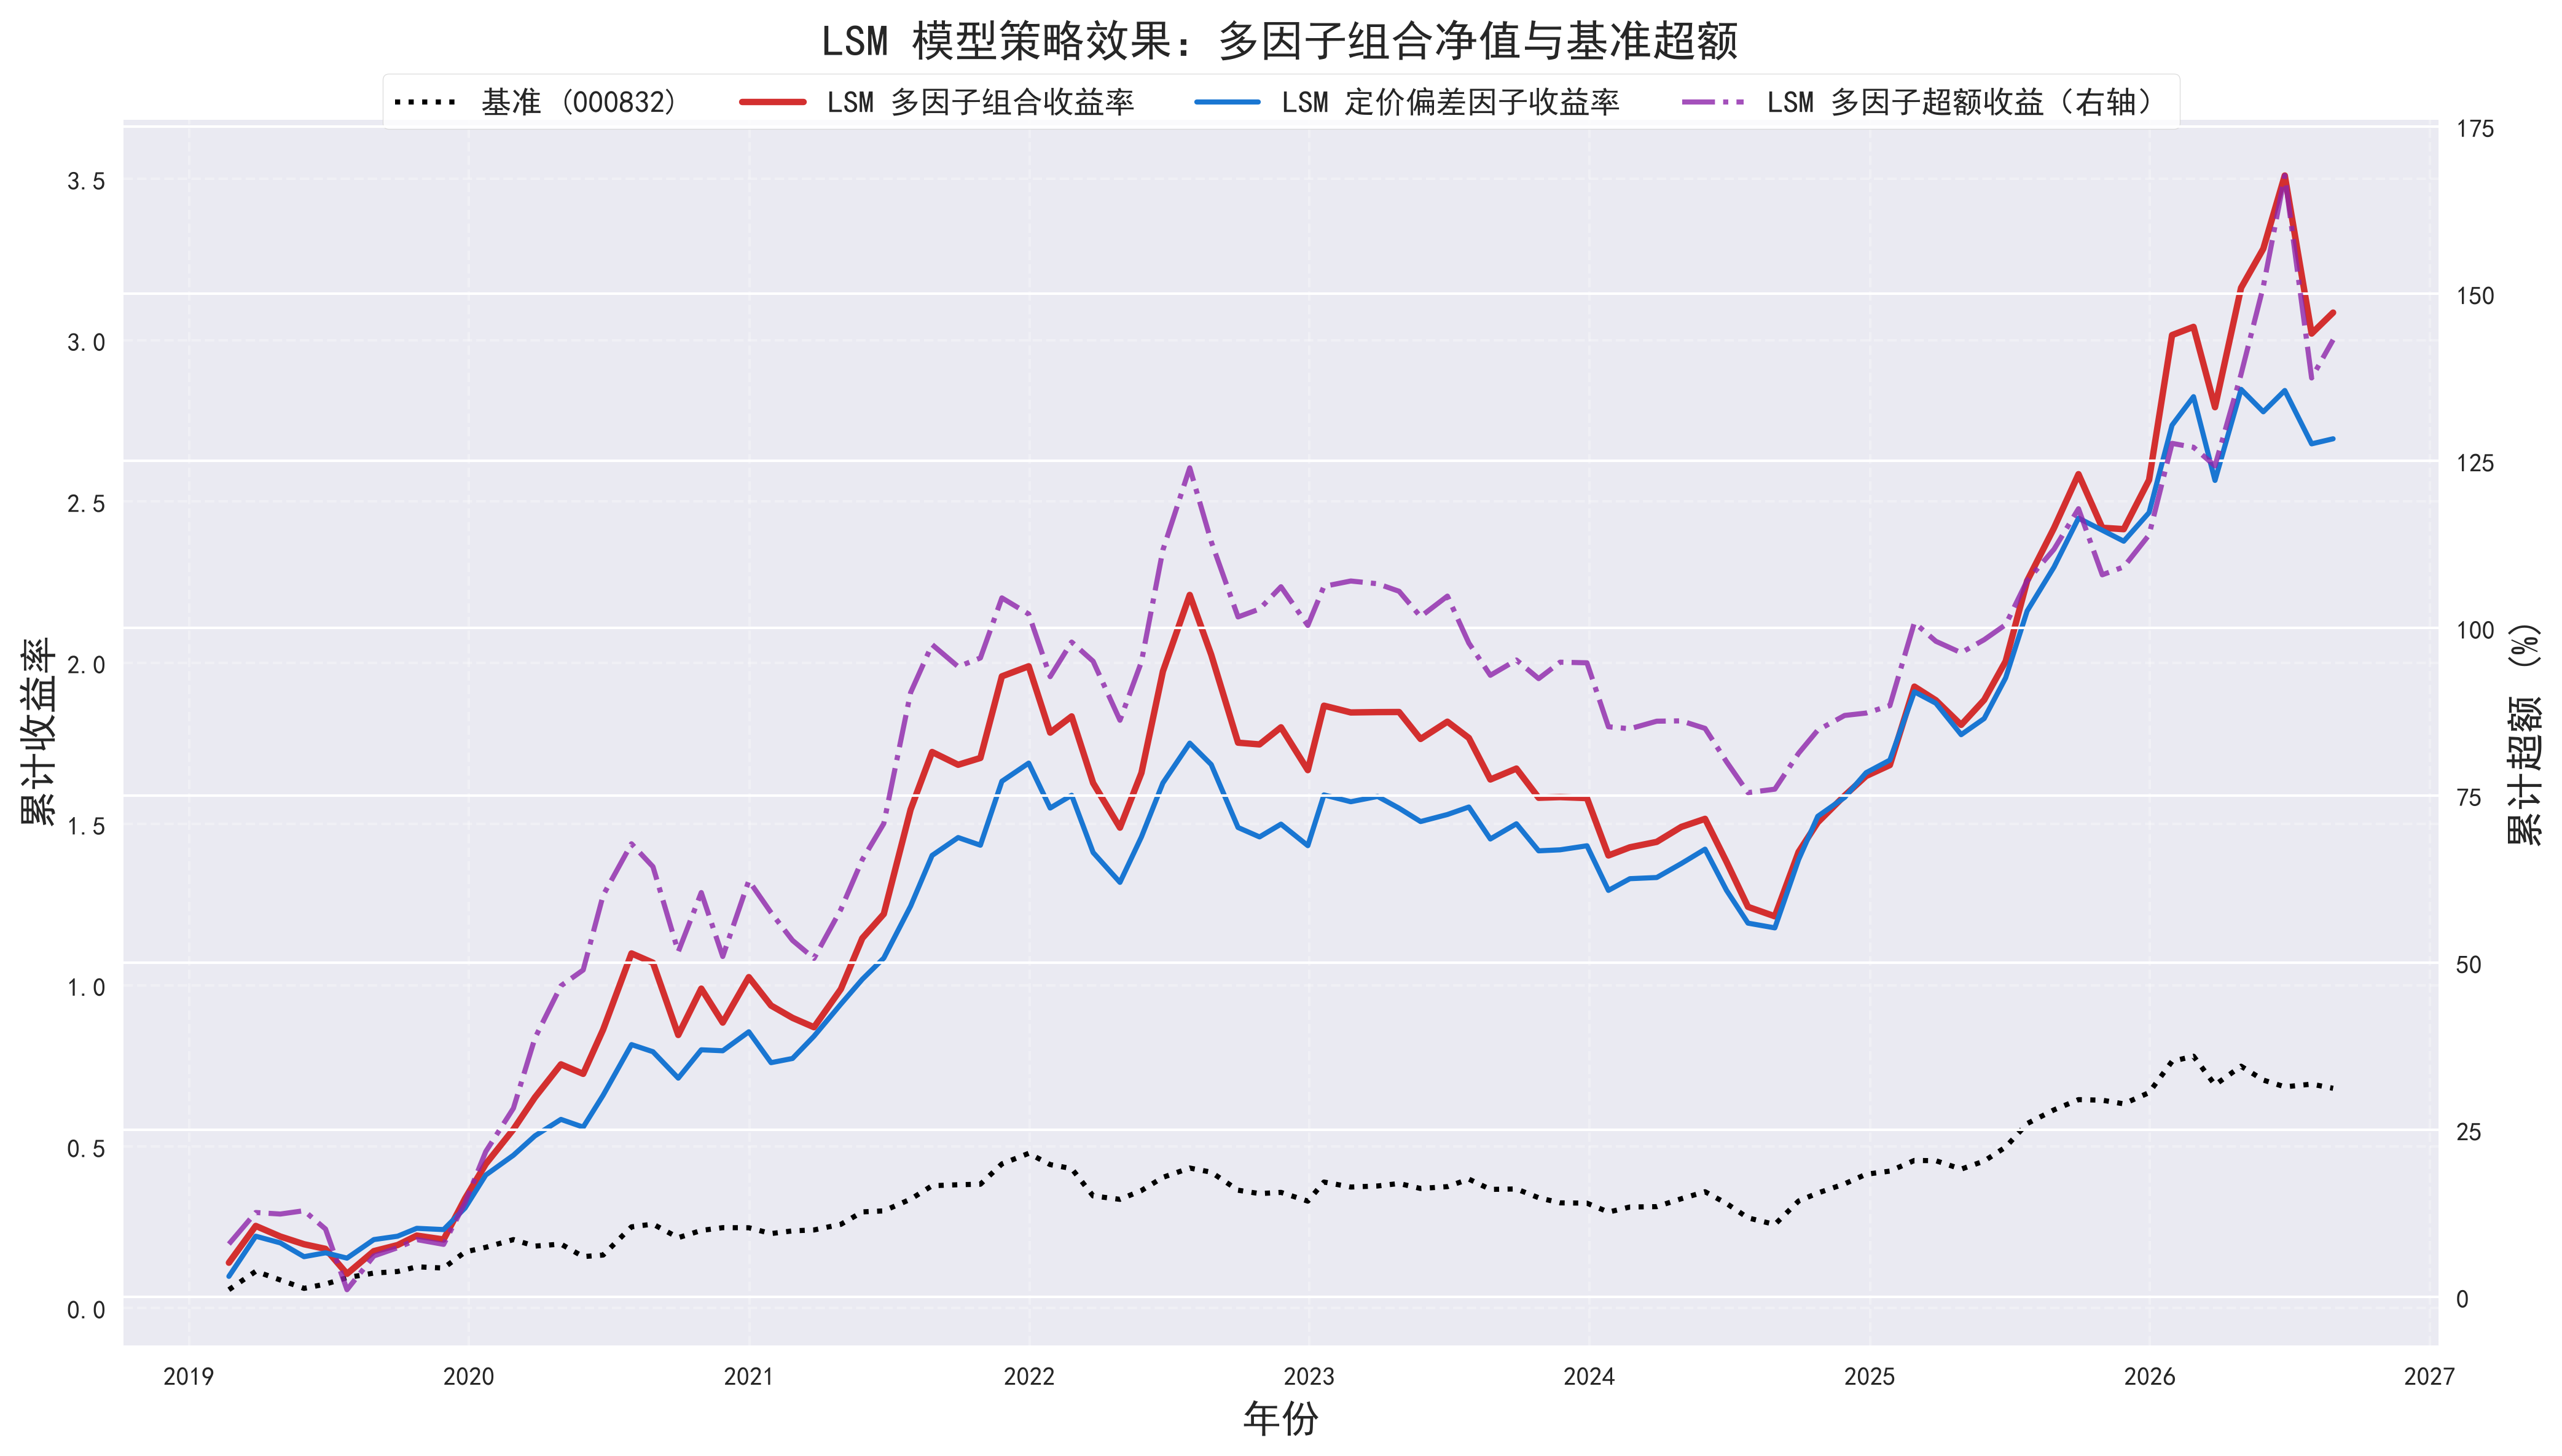
\includegraphics[width=0.76\textwidth]{../long-short strategy/LSM_model_performance.png}
  \caption{LSM 定价偏差策略与基准净值}
\end{figure}

\clearpage
\sectionbar{四、因子关系与解释边界}

因子冗余同时使用 Pearson 线性相关与 Spearman 秩相关检验。估值因子先调整
方向，使所有因子的数值越高都代表预期收益越高。定价偏差与流动性、动量和
量价因子的关系较弱，但与估值因子有明显重合，因而不能将定价信号描述为
与传统估值正交。

\begin{table}[h!]
  \centering
  \caption{定价偏差与估值因子的相关性}
  \begin{tabular}{lrr}
    \toprule
    模型 & Pearson & Spearman \\
    \midrule
    BS  & 0.558 & 0.612 \\
    ZL  & 0.535 & 0.683 \\
    LSM & 0.465 & 0.571 \\
    \bottomrule
  \end{tabular}
\end{table}

预测检验把每个月末的因子值只与下一持有期的单券收益配对，并在每个模型内
保留六因子数据完整且通过交易筛选的共同截面。2019-01-25 至 2026-08-28
共有 91 个可检验持有期。下表的 ICIR 与 Rank ICIR 为逐期均值除以逐期标准差，
未作年化。

\begin{table}[h!]
  \centering
  \caption{逐因子 IC 与 Rank IC 汇总}
  \scriptsize
  \setlength{\tabcolsep}{3.3pt}
  \begin{tabular}{llrrrrr}
    \toprule
    模型 & 因子 & IC & Rank IC & ICIR & Rank ICIR & IC 为正 \\
    \midrule
    BS & 流动性 & -0.021 & -0.070 & -0.10 & -0.39 & 46.2\% \\
       & 波动率 & -0.016 & -0.069 & -0.06 & -0.26 & 45.1\% \\
       & 量价 & -0.003 & -0.058 & -0.02 & -0.37 & 47.3\% \\
       & 估值 & 0.047 & 0.057 & 0.24 & 0.33 & 61.5\% \\
       & 动量 & 0.017 & -0.010 & 0.09 & -0.06 & 59.3\% \\
       & 定价偏差 & 0.077 & 0.044 & 0.48 & 0.27 & 65.9\% \\
    \midrule
    ZL & 流动性 & -0.018 & -0.071 & -0.08 & -0.36 & 47.3\% \\
       & 波动率 & -0.019 & -0.071 & -0.07 & -0.28 & 49.5\% \\
       & 量价 & -0.005 & -0.058 & -0.03 & -0.35 & 45.1\% \\
       & 估值 & 0.049 & 0.059 & 0.25 & 0.34 & 64.8\% \\
       & 动量 & 0.017 & -0.012 & 0.08 & -0.08 & 58.2\% \\
       & 定价偏差 & 0.096 & 0.081 & 0.50 & 0.51 & 72.5\% \\
    \midrule
    LSM & 流动性 & -0.018 & -0.071 & -0.08 & -0.36 & 47.3\% \\
        & 波动率 & -0.019 & -0.071 & -0.07 & -0.28 & 49.5\% \\
        & 量价 & -0.005 & -0.058 & -0.03 & -0.35 & 45.1\% \\
        & 估值 & 0.049 & 0.059 & 0.25 & 0.34 & 64.8\% \\
        & 动量 & 0.017 & -0.012 & 0.08 & -0.08 & 58.2\% \\
        & 定价偏差 & 0.076 & 0.051 & 0.50 & 0.34 & 65.9\% \\
    \bottomrule
  \end{tabular}
\end{table}

\begin{figure}[h!]
  \centering
  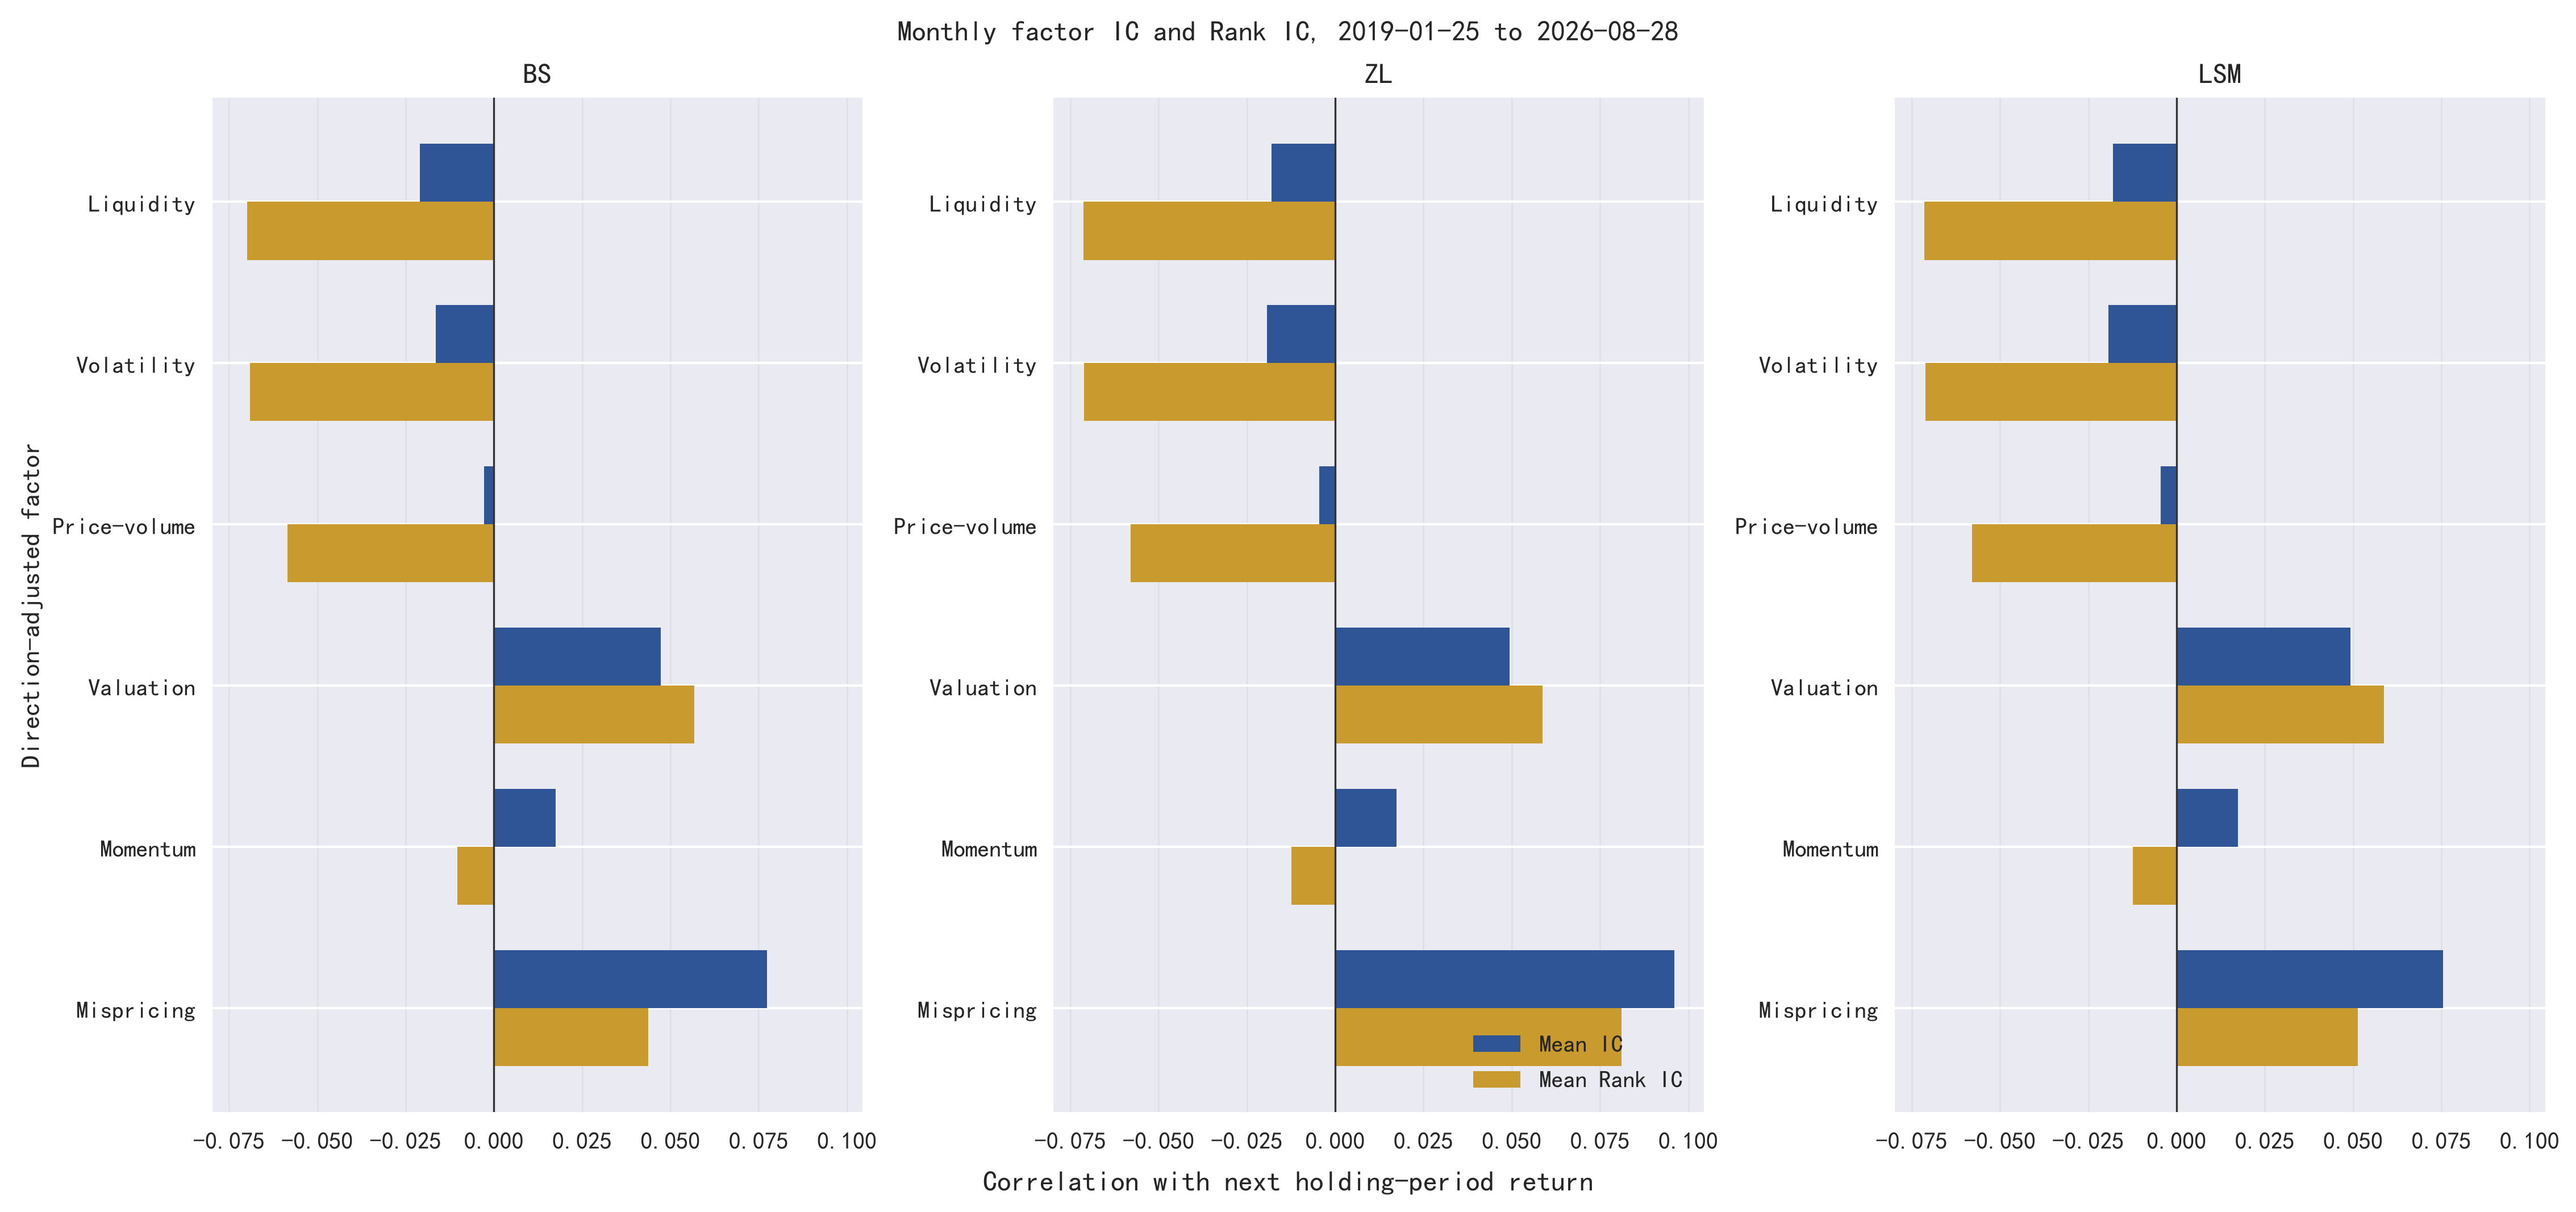
\includegraphics[width=0.94\textwidth]{../mispricing factor/factor_ic_comparison.png}
  \caption{三种模型六因子的平均 IC 与 Rank IC}
\end{figure}

ZL 定价偏差的预测关系最稳定，平均 IC 为 0.096，平均 Rank IC 为 0.081，
两者为正的比例分别为 72.5\% 和 70.3\%。估值因子也呈正预测关系，流动性、
波动率与量价因子的平均 Rank IC 则为负。这个结果与定价偏差单因子策略优于
机械六因子等权组合的表现一致，但仍属于样本内描述，不能作为因果证据。

\clearpage
\sectionbar{五、数据与复现口径}

\begin{tabularx}{\textwidth}{>{\bfseries}p{3.2cm}X}
  \toprule
  项目 & 当前口径 \\
  \midrule
  市场数据 & Tushare 可转债日行情、基础信息、评级、财务指标及正股数据；
             AkShare 国债收益率曲线。 \\
  模型观察频率 & 每个已完成交易周保留一个实际交易日定价截面。 \\
  策略调仓 & 月末调仓，收益期从 2019-01-25 开始，最后一个观察期结束于
             2026-08-28。 \\
  交易成本 & 多头因子回测扣除双边 0.06\% 交易成本。 \\
  夏普口径 & 使用回测期内实际观测的一年期国债收益率均值作为无风险利率。 \\
  输出依据 & \texttt{BS/ZL/LSM\_Model\_Summary.xlsx}、
             \texttt{B-S/Z-L/LSM\_alpha\_strategy\_results.csv}、因子相关性矩阵、
             逐期 IC/Rank IC 列表及其 Manifest。 \\
  增量约束 & 日常周更新从 \texttt{ZL\_Model\_Manifest.json} 读取已验证截止日，
             LSM 使用独立 Manifest；各模型只定价后续新增交易周。 \\
  \bottomrule
\end{tabularx}

\sectionbar{六、LSM 模型实现}

东北证券《可转债研究框架：从理论概念到实战策略》还介绍了第三种绝对定价
方法 LSM（最小二乘蒙特卡罗）。LSM 通过回归估计继续持有价值，并与即时转股
价值比较，以处理美式提前转股权。

本仓库已按东北证券报告的二次基函数 $1,S,S^2$ 实现批量向量化 LSM。
生产参数为 256 条对偶路径、48 个行权时点与按日期固定的随机种子。
到期收益取转股价值与到期赎回价之较大者；回溯时比较即时转股与回归继续价值。
为避免与 ZL 中已含的转股权重复加总，组合价格取两个独立价值的较大者。
首轮历史回测覆盖 392 个周度截面和 138,820 个定价样本；后续运行由
\texttt{LSM\_Model\_Manifest.json} 校验参数、历史输入指纹和输出哈希，严格只算新增日期。

\sectionbar{七、结论与证据边界}

\begin{itemize}
  \item 模型价格依赖波动率、信用利差和条款行为假设，参数误差可能形成长期、
        不可收敛的定价偏离。
  \item 中国可转债卖空和对冲机制有限，理论高估不等于可实现的空头收益。
  \item 回测存在样本内选择、存续样本结构变化、流动性和容量约束。
  \item IC、Rank IC 及其显著性统计是样本内描述；因子相关性也不等同于因果识别。
  \item 当前结果支持将 BS、ZL 与 LSM 作为互补定价锚，但仍需风险预算、市场状态
        约束和样本外检验。
\end{itemize}

当前证据支持把 BS、ZL 与 LSM 视为互补的估值工具。BS 提供透明的权益端基准，
ZL 体现条款与债券现金流，LSM 补充继续价值和自愿提前转股。研究结果同时说明，
模型复杂度需要由多维证据约束。价格误差、组合收益和风险表现并不随复杂度单调改善。

\end{document}
